\documentclass[submission,copyright,creativecommons]{eptcs}
%\providecommand{\event}{SOS 2007} % Name of the event you are submitting to
\usepackage{breakurl}             % Not needed if you use pdflatex only.
\usepackage{datetime}
\newdate{date}{04}{18}{2018}
\date{\displaydate{date}}
\usepackage{graphicx} %package to manage images
\graphicspath{ {images/} }

\usepackage[rightcaption]{sidecap}

\usepackage{wrapfig}
\title{Blockchain principles applied to transaction operations on the Real Estate Market}
\author{Andres Salgado
\institute{International Technological University\\ San Jose, California, \underline{USA}}
\email{salgadoandre533@students.itu.edu}
\and
Co Authors \qquad\qquad Jorge Valdeiglesias, Kartikeya Yellayi
\institute{International Technological University\\ San Jose, California, \underline{USA}}
\email{\quad valdeiglesjorge744@students.itu.edu \quad\qquad yellayishiva1284@students.itu.edu}
}

\def\titlerunning{Blockchain principles applied to transaction operations on the Real Estate Market}
\def\authorrunning{R.J. van Glabbeek, C. Author \& Y.S. Else}

\begin{document}
\maketitle
\displaydate{date}

\begin{abstract}
This is a sentence in the abstract.
This is another sentence in the abstract.
This is yet another sentence in the abstract.
This is the final sentence in the abstract.
\end{abstract}

\section{Introduction}

With the advent of ``blockchain'' technologies, as well as the necessity to establish a system where the trust of transactions could be offloaded to machines, we ventured into exploring how a system based on the Ethereum blockchain could accurately execute a series of smart contracts in order to validate a transaction between two entities.

%By means of the style-file option
%\href{http://creativecommons.org/about/license/}{creativecommons}
%authors equip their paper with a Creative Commons license that allows
%everyone to copy, distribute, display, and perform their copyrighted
%work and derivative works based upon it, but only if they give credit%the way you request. By invoking the additional style-file option {\tt
%noderivs} you let others copy, distribute, display, and perform only
%verbatim copies of your work, but not derivative works based upon
%it. Alternatively, the {\tt sharealike} option allows others to
%distribute derivative works only under a license identical to the
%license that governs your work. Finally, you can invoke the option
%{\tt noncommercial} that let others copy, distribute, display, and
%perform your work and derivative works based upon it for
%noncommercial purposes only.


\section{The blockchain and its influence on crypto-currencies}

It's close to 10 years after Bitcoin was introduced by Satoshi Nakamoto. The reason crypto-currencies currently exist is due to the underlying technology made available by the blockchain. Thomas Lowenthal from Ars Technica \cite{lowenthalBitcoinEncryptedPeertopeer2011} goes onto explaining the complexities of cryptographic currencies, the concept of mining and make-work, and goes onto comparing Bitcoin against the trusty greenback which also faced hurdles when it was first put into circulation.

The primary reason why cryptocurrencies are being adopted by a sizable portion of the population is due to the engineering concept behind the implementation of the blockchain to solve two basic problems inherit to digital currencies, the double-spending problem, and the prevention of counterfeiting\cite{noauthor_bitcoin}.
On cppcon 2016 David Schwarz\cite{cppconCppCon2016David} spoke about "Developing Blockchain Software".  On his talk he mentions key characteristics of "the blockchain". Section 2.1 goes onto describing such characteristics.   

\subsection{What is a blockchain and what is one good for?}
\begin{itemize}
\item Blockchains record state and history
\item State is modified by transactions
\item Everyone eventually agrees on the transactions
\item Can be used to transfer tokens
\end{itemize}

Based on this list, most of us would conclude that the blockchain is merely a database, but in actuality, the blockchain -according to Schwarz\cite{cppconCppCon2016David}- manages the double-spending problem.

\subsection{What the blockchain does for bitcoin}

Figure 1 describes how the blockchain validates bitcoin as cryptocurrency system\cite{noauthor_bitcoin}
\begin{figure}[h]
    \centering
    \label{fig:my_label}
    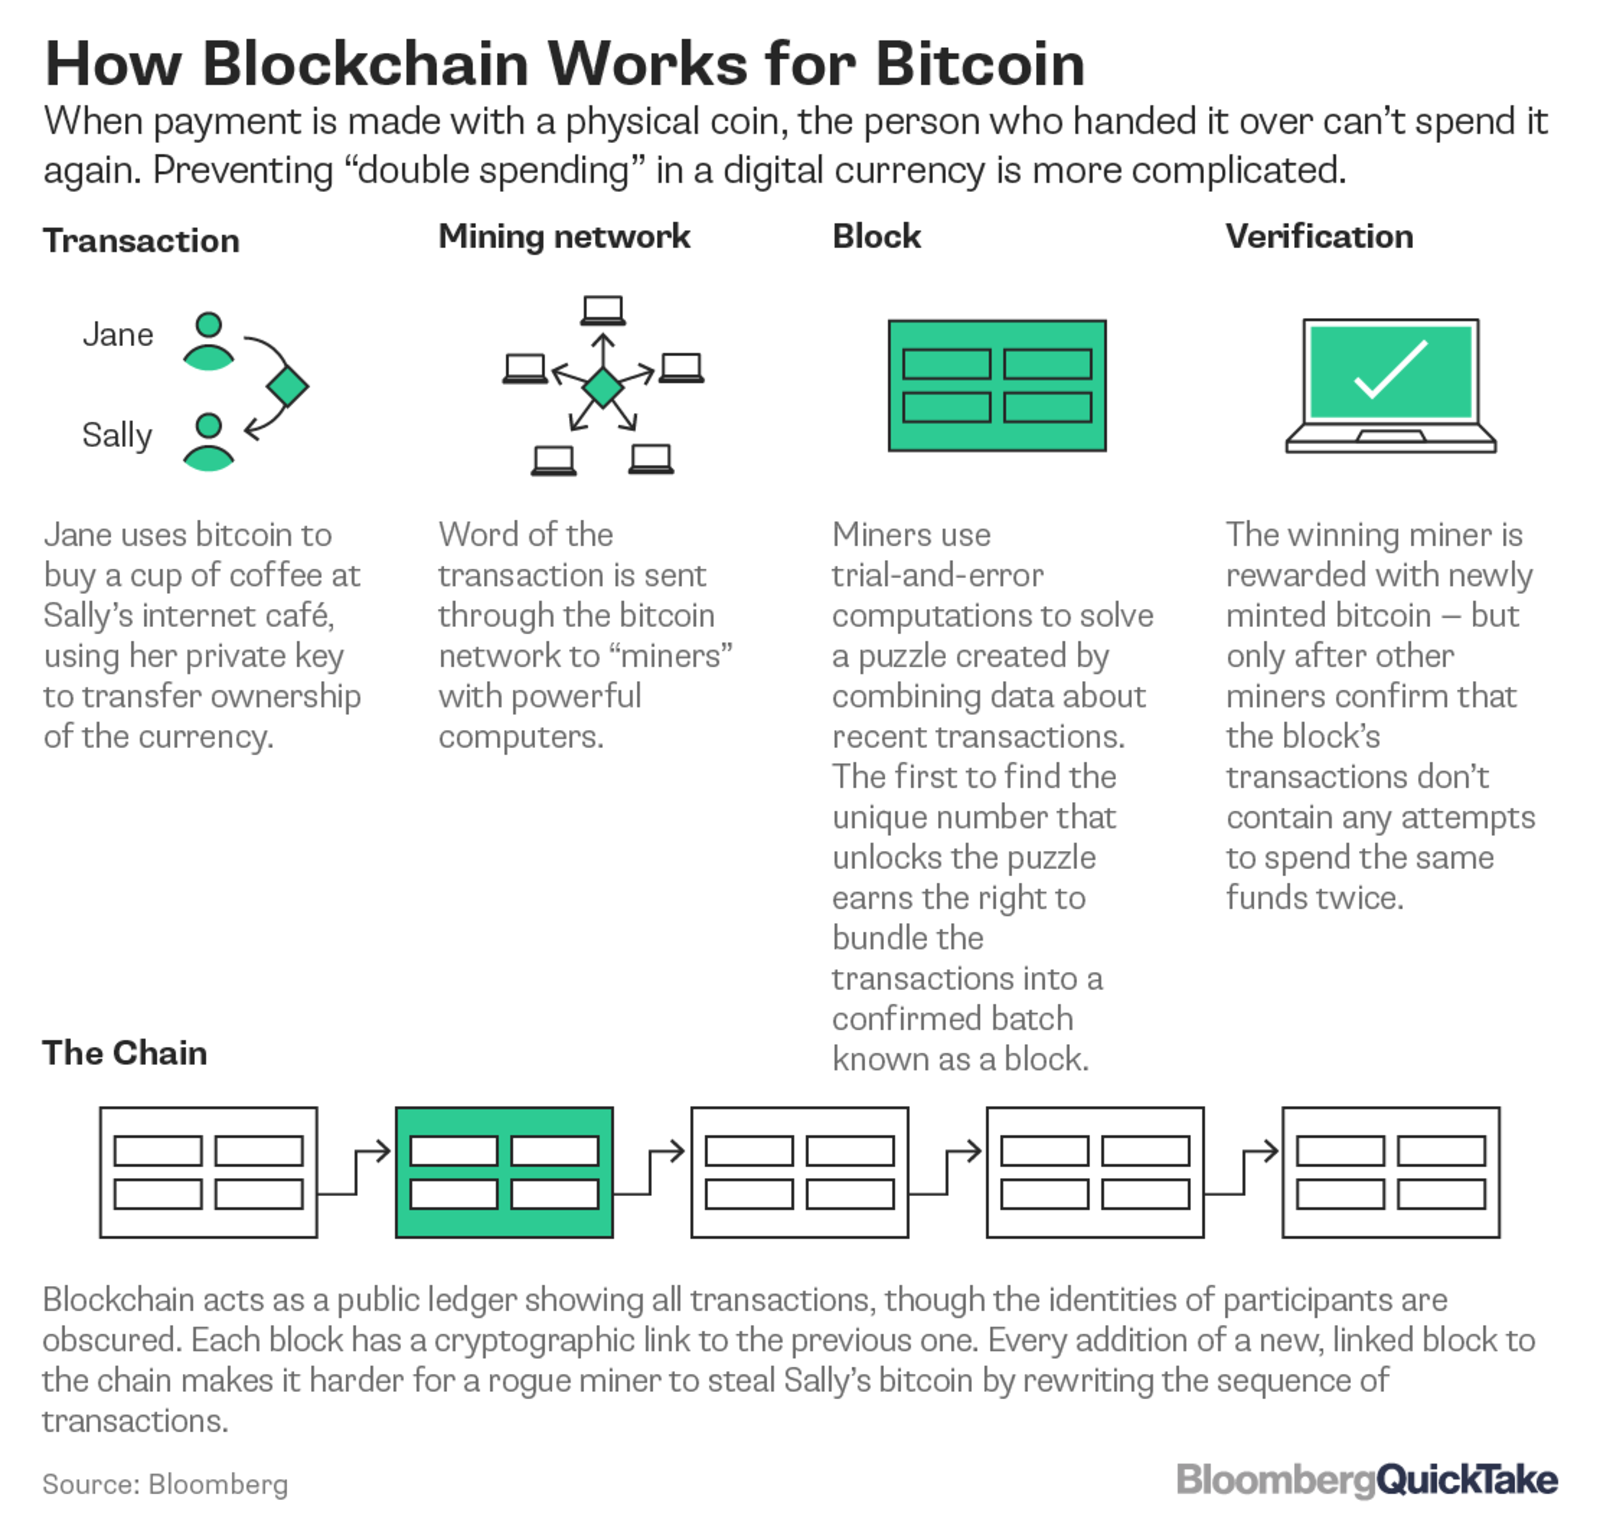
\includegraphics[width=5in]{bitcoin-blockchain-bloomberg}
     \caption{Image Source: BloombergQuicktake}
\end{figure}.


\section{Beyond Bitcoin (other industries and its use)}
Besides solving the issue of how to allow for a feasible digital currency, the blockchain has opened the door towards the development of new uses of the technology, that do not necessarily address the exchange of assets in a digital manner.  This exposure has allowed millions of dollars to be poured into research and development of proper blockchain applications in a variety of fields with distinct uses and outcomes.
One of the business that seems to be benefiting the most from this investments is the logistics business. Many companies are involved in the process of carrying goods. Most importantly, because there are several actors involved in such process, a delay in shipment can prove to be catastrophic to huge shipments.  

Currently the majority of companies that engage in gathering data to make business decisions use different types of database systems in order to store, query and build statistical model out of collected data.  When the interaction with that data doesn't require sharing such information, companies are equipped to process it, but when two or more entities\cite{BlockchainGoesCryptoCurrency2016} need to share such data, it is often complicated to achieve a consensus on how such exchange should be handled.\footnote{Olga Kharif on her article "Blockchain Goes Beyond Crypto-Currency" explains how companies in Finland, Sweden, Estonia and Latvia are beginning to use a blockchain system in order to share information. }


\section{Bibliography}




\bibliographystyle{unsrt}
\bibliography{biblio}
%\listoffigures
\end{document}
